% !TeX program = xelatex
\documentclass[UTF8,11pt,a4paper,fontset=fandol]{ctexart}
\usepackage[margin=2.5cm]{geometry}
\usepackage{amsmath,amssymb,amsthm,bm,mathtools}
\usepackage{graphicx,booktabs,array,tikz}
\usepackage{needspace}
\usetikzlibrary{arrows.meta,calc,intersections,positioning}
\usepackage[colorlinks=true,linkcolor=blue,urlcolor=blue,citecolor=blue]{hyperref}
\numberwithin{equation}{section}
\newtheorem{theorem}{定理}[section]
\newtheorem{lemma}[theorem]{引理}
\newtheorem{corollary}[theorem]{推论}
\renewcommand{\proofname}{证明}
\newcommand{\dd}{\,\mathrm d}
\newcommand{\cross}[2]{[#1,#2]}
\tikzset{proofpic/.style={font=\fontsize{12}{14}\selectfont,>=Stealth},
 edge/.style={draw=black!75,line width=1.5pt},
 front/.style={draw=blue!70!black,line width=2.2pt},
 rayline/.style={draw=black!50,line width=1pt},
 event/.style={draw=orange!85!black,dashed,line width=1.3pt},
 point/.style={circle,draw=black,fill=white,inner sep=1.6pt,line width=1pt}}
\title{精确波前积分中几何操作的正确性与完备性}
\author{王廷骥}
\date{2026年11月9日}
\begin{document}
\maketitle
\noindent\textbf{要证明的结论。}
对于平面凸四边形和任意有限组同心圆，只需收集\textbf{顶点方向与圆、边交点方向}，再在相邻方向之间进行径向裁剪，就能覆盖全部待积分区域，且各子区内部不重叠。证明的关键不是列全图形，而是证明：\textbf{除此之外，不存在使边界关系改变的位置。}

\section{用有向面积统一表示单元}
将同心圆的圆心移到原点 $O$。设 $Q$ 为具有非空内部的闭凸四边形，顶点 $\bm{a}_1,\ldots,\bm{a}_4$ 按逆时针排列，$\bm{a}_5=\bm{a}_1$，各边非零。记
\[
 \bm{e}_i=\bm{a}_{i+1}-\bm{a}_i,\qquad
 \cross{\bm{u}}{\bm{v}}=u_xv_y-u_yv_x.
\]
本文用粗体表示向量，向量的分量及半径、角度等标量采用普通斜体。$\cross{\bm{u}}{\bm{v}}/2$ 就是由位置向量 $\bm{u},\bm{v}$ 与原点 $O$ 确定的三角形的有向面积；若记对应复数为 $z_u=u_x+\mathrm{i}u_y$、$z_v=v_x+\mathrm{i}v_y$，则 $\cross{\bm{u}}{\bm{v}}=\operatorname{Im}(\overline{z_u}z_v)$。以下采用向量写法。

凸四边形恰为四条有向边左侧闭半平面的交：
\begin{equation}\label{eq:halfplane}
 Q=\bigcap_{i=1}^{4}\{\bm{x}:\cross{\bm{e}_i}{\bm{x}-\bm{a}_i}\geq0\}.
\end{equation}
这是凸多边形的支撑半平面表示：每条边的左侧都包含 $Q$；这些相邻边围成的有界交集又恰以 $\bm{a}_i$ 为顶点，故交集就是 $Q$。因此式 \eqref{eq:halfplane} 同时适用于圆心位于单元内、外、边上或顶点上的情况。

对方向 $\bm{d}(\theta)=(\cos\theta,\sin\theta)$，将射线 $\bm{x}=\rho \bm{d}(\theta)$、$\rho\geq0$ 代入，得到
\begin{equation}\label{eq:ray}
 D_i(\theta)\rho\geq c_i,\qquad
 D_i(\theta)=\cross{\bm{e}_i}{\bm{d}(\theta)},\quad c_i=\cross{\bm{e}_i}{\bm{a}_i}.
\end{equation}
于是射线上的单元区间由下列规则精确给出：
\begin{equation}\label{eq:bounds}
 \ell(\theta)=\max\left(\{0\}\cup\left\{\frac{c_i}{D_i}:D_i>0\right\}\right),
 \qquad
 u(\theta)=\min\left\{\frac{c_i}{D_i}:D_i<0\right\}.
\end{equation}
空集的最小值约定为 $+\infty$。若某个 $D_i=0$ 且 $c_i>0$，射线与单元不相交；若 $D_i=0$ 且 $c_i\leq0$，该约束自动满足。其余情况下，$u\geq\ell$ 时交集为 $[\ell,u]$，$u<\ell$ 时为空。单元有界，故非空交集的上端点有限。

\textbf{这一步已经保证径向裁剪没有遗漏：}每条边只提供一个上界、下界或可行性条件；取交集即可，不需要先判断圆心属于哪一类位置。

\begin{figure}[htbp]
\centering
\begin{tikzpicture}[proofpic,x=1.2cm,y=1.2cm]
 \fill[blue!7] (1,-.65) rectangle (4,1.25);
 \draw[edge] (1,-.65)--(4,-.65)--(4,1.25)--(1,1.25)--cycle;
 \draw[edge,->] (1,-.65)--(2.7,-.65);
 \node[below] at (1,-.65) {$\bm{a}_i$};
 \node[below] at (4,-.65) {$\bm{a}_{i+1}$};
 \node[below] at (2.5,-.65) {$\bm{e}_i$};
 \node at (2.5,.85) {$[\bm{e}_i,\bm{x}-\bm{a}_i]\geq0$};
 \draw[rayline,->] (0,0)--(5.25,0) node[right] {$\bm{d}(\theta)$};
 \draw[front] (1,0)--(4,0);
 \node[point,label=below:$O$] at (0,0) {};
 \node[point,label=below:$\ell \bm{d}$] at (1,0) {};
 \node[point,label=below:$u \bm{d}$] at (4,0) {};
 \node[above] at (2.5,0) {$Q\cap\{\rho \bm{d}:\rho\geq0\}$};
 \draw[->,line width=1pt] (4.8,.48)--(3.8,.48);
 \node[above] at (4.8,.48) {从外向内};
\end{tikzpicture}
\caption{有向边的左侧约束与射线交区间。蓝色线段是四个半平面约束的共同解。从远处沿射线向内，依次经历“单元外、单元内、单元外”，这也是引理\ref{lem:edge}采用的判断方式。}
\label{fig:halfplane}
\end{figure}

\section{为什么只需要两类分割方向}
取全部需要使用的半径，排序、去重后记为
\[
 0=r_0<r_1<\cdots<r_m.
\]
其中包含积分支撑的内、外半径及所有核函数分段半径；也可加入为提高积分精度而设置的辅助半径。暂以 $S=Q\cap\{|\bm{x}|\leq r_m\}$ 为目标区域；若支撑为圆环，只保留对应的径向带即可。

定义角度集合
\begin{equation}\label{eq:events}
 \mathcal E=\{0,2\pi\}
 \cup\{\arg \bm{a}_i:\bm{a}_i\ne\bm{0}\}
 \cup\{\arg \bm{p}:\bm{p}\in\partial Q,\ |\bm{p}|=r_j,\ j\geq1\},
\end{equation}
非零点的辐角取在 $[0,2\pi)$。将这些角度排序、去重，记为
$0=\theta_0<\theta_1<\cdots<\theta_N=2\pi$，并称
$J_k=(\theta_k,\theta_{k+1})$ 为一个开角区间。

图\ref{fig:events}分别展示两种变化：经过顶点时，提供端点的边可能改变；经过圆、边交点时，端点与圆半径的大小关系可能改变。以下两条引理证明这两类方向已经足够。
\begin{figure}[htbp]
\centering
\begin{tikzpicture}[proofpic,x=1.35cm,y=1.35cm]
 \begin{scope}
  \fill[blue!5] (1,-.4) rectangle (3,2);
  \draw[edge] (1,-.4) rectangle (3,2);
  \draw[rayline,->] (0,0)--(3.65,0);
  \draw[rayline] (0,0)--(3.45,1.61);
  \draw[rayline] (0,0)--(2.75,2.75);
  \draw[event] (0,0)--(3.6,2.4);
  \node[point,label=below:$O$] at (0,0) {};
  \node[point,label=right:$\bm{a}_i$] at (3,2) {};
  \node[point] at (3,1.399) {};
  \node[point] at (2,2) {};
  \node[above] at (1.65,2.05) {上边退出};
  \node[right] at (3.05,.85) {右边退出};
  \node at (1.9,-.95) {（a）顶点方向};
 \end{scope}
 \begin{scope}[xshift=7.6cm]
  \fill[blue!5] (1,-.4) rectangle (3,2);
  \draw[edge] (1,-.4) rectangle (3,2);
  \draw[front] (0:3.2) arc (0:48:3.2);
  \draw[rayline,->] (0,0)--(3.6,0);
  \draw[rayline] (0,0)--(3.5,{3.5*tan(10)});
  \draw[rayline] (0,0)--(3.5,{3.5*tan(30)});
  \draw[event] (0,0)--(3.6,{3.6*sqrt(1.24)/3});
  \node[point,label=below:$O$] at (0,0) {};
  \node[point,label=right:$\bm{p}$] at (3,{sqrt(1.24)}) {};
  \node[above] at (2.25,2.25) {$\rho=r_j$};
  \node[fill=white,inner sep=1pt] at (1.9,.32) {$u<r_j$};
  \node[fill=white,inner sep=1pt] at (1.8,1.4) {$u>r_j$};
  \node at (1.9,-.95) {（b）圆、边交点方向};
 \end{scope}
\end{tikzpicture}
\caption{两类分割方向的作用。橙色虚线是发生变化的方向，灰线是其两侧的射线；图（b）中 $\bm{p}$ 满足 $u=r_j$。这里只标出用于说明变化的射线，完整分割需收集所有顶点和所有圆、边交点。}
\label{fig:events}
\end{figure}

两条引理分别回答两个问题：\textbf{射线在单元中的那一段由哪些边确定？圆环又从这一段中留下哪一部分？}这里“不变”指边的身份和端点的大小顺序不变，并不是端点的数值不变。

\Needspace{7\baselineskip}
\begin{lemma}[不越过顶点方向，射线穿过的边就不变]\label{lem:edge}
让射线在一个不含任何顶点方向的开角区间内连续转动。则它穿过哪些边、按什么顺序穿过，都不会改变，各交点沿相应的边连续移动。因此，射线在单元内的正长度区间要么始终不存在，要么始终存在；存在时，其下端点 $\ell(\theta)$ 始终由同一条边或原点确定，上端点 $u(\theta)$ 始终由同一条边确定。
\end{lemma}
\begin{proof}
\textbf{先看一条边。}如图\ref{fig:lemma-edge}（a），一条不过原点的直边对应一段连续的方向范围，两端就是顶点方向。这个结论可由有向面积直接验证：令
$\bm{p}(t)=\bm{a}_i+t\bm{e}_i$，$0\leq t\leq1$，则
\begin{equation}\label{eq:anglederivative}
 \frac{\dd}{\dd t}\arg\bm{p}(t)
 =\frac{[\bm{p}(t),\bm{e}_i]}{|\bm{p}(t)|^2}
 =-\frac{c_i}{|\bm{p}(t)|^2}\ne0.
\end{equation}
导数的符号固定，所以沿边移动时方向只向一侧变化，不会折返。故射线只要没有越过两个端点的方向，就不会突然与这条边相交或突然不再相交；相交时，交点半径 $c_i/D_i(\theta)$ 连续变化。辐角跨越 $2\pi$ 时在 $0$ 方向处分开即可。

若边所在直线经过原点，边上的非零点仅位于一条或两条固定射线上，方向由非零端点给出。这些方向已被排除，因而该边不会在开角区间内部产生交点。

\textbf{再把各条边合起来。}两个边界交点若交换先后顺序，中间就必须重合；不同边只能在公共顶点相交，而顶点方向已被排除。因此交点的数目、所属边和顺序均不变。

最后，从足够远处沿射线向原点移动，起初必在单元外，每穿过一个边界交点就切换一次内外状态，见图\ref{fig:lemma-edge}（b）。这些交点既不在顶点上，也不沿边，故都是穿过而非擦过。凸性保证最多有两个正的交点：无交点时没有正长度交区间；一个交点时区间为 $[0,u]$；两个交点时区间为 $[\ell,u]$。于是区间是否存在以及端点由谁确定，都不再改变。
\end{proof}

\begin{figure}[htbp]
\centering
\begin{tikzpicture}[proofpic,x=1.25cm,y=1.25cm]
 \begin{scope}
  \fill[blue!8] (0,0)--(3,.4)--(3,2.2)--cycle;
  \draw[event] (0,0)--(3.3,.44);
  \draw[event] (0,0)--(3.3,2.42);
  \draw[rayline] (0,0)--(3,1);
  \draw[rayline] (0,0)--(3,1.6);
  \draw[edge,->] (3,.4)--(3,2.2);
  \node[point,label=below:$O$] at (0,0) {};
  \node[point,label=right:$\bm{a}_i$] at (3,.4) {};
  \node[point,label=right:$\bm{a}_{i+1}$] at (3,2.2) {};
  \node[point] at (3,1) {};
  \node[point] at (3,1.6) {};
  \draw[->,line width=1pt] (2.7,1.05)--(2.7,1.55);
  \node at (1.65,-.55) {（a）交点沿同一条边移动};
 \end{scope}
 \begin{scope}[xshift=7.2cm]
  \fill[blue!7] (1,.5) rectangle (3,2);
  \draw[edge] (1,.5) rectangle (3,2);
  \draw[rayline,->] (0,1)--(4.2,1) node[right] {$\rho$};
  \draw[front] (1,1)--(3,1);
  \node[point,label=below:$O$] at (0,1) {};
  \node[point,label=below:$\ell$] at (1,1) {};
  \node[point,label=below:$u$] at (3,1) {};
  \node at (.5,1.4) {外};
  \node at (2,1.4) {内};
  \node at (3.7,1.4) {外};
  \draw[->,line width=1pt] (4,2.35)--(2.7,2.35);
  \node[above] at (3.3,2.35) {从远处向内};
  \node at (2,-.55) {（b）穿过边界时切换内外};
 \end{scope}
\end{tikzpicture}
\caption{引理\ref{lem:edge}的两个证明步骤。先确定每条边对应的方向范围，再根据交点顺序确定单元内的径向区间。图（b）中的 $\ell,u$ 是交点的径向坐标，均为标量。}
\label{fig:lemma-edge}
\end{figure}

\begin{lemma}[不越过圆、边交点方向，圆环的截取方式就不变]\label{lem:structure}
在相邻分割方向之间的 $J_k$ 内，若单元交区间 $[\ell(\theta),u(\theta)]$ 存在，则每个端点与每个圆半径 $r_j$ 的大小关系固定。于是，对任一径向带 $[r_j,r_{j+1}]$，其与单元区间的交集要么始终没有正长度，要么始终具有正长度；后一种情况下，下限始终取自 $\ell$ 或 $r_j$ 中的同一个，上限始终取自 $u$ 或 $r_{j+1}$ 中的同一个。
\end{lemma}
\begin{proof}
\textbf{端点要从圆内走到圆外，必先经过圆周。}由引理\ref{lem:edge}，正的端点沿某条固定的边连续移动。若它与 $r_j$ 的大小关系改变，中途必有 $\ell=r_j$ 或 $u=r_j$，对应点就是圆、边交点。然而该交点的方向已经用于切分，不可能落在 $J_k$ 内。因此大小关系不变；若下端点是原点，则 $\ell=0<r_j$ 对所有正半径自动成立。

\textbf{大小顺序固定，取交集的方式也就固定。}两个区间的交集下限取较大者，上限取较小者，即
\[
 [\ell,u]\cap[r_j,r_{j+1}]
 =[\max\{\ell,r_j\},\min\{u,r_{j+1}\}],
\]
右端小于左端时按空集处理。由于 $\ell<u$、$r_j<r_{j+1}$，交集有正长度恰好等价于
\[
 \ell<r_{j+1}\quad\text{且}\quad r_j<u.
\]
这些比较关系在整个 $J_k$ 内均不变，所以交集不会在区间中途出现或消失，下、上限的来源也不会改变。图\ref{fig:lemma-clip}给出其中一种固定顺序，其他顺序由同一组最大值、最小值公式处理。
\end{proof}

\begin{figure}[htbp]
\centering
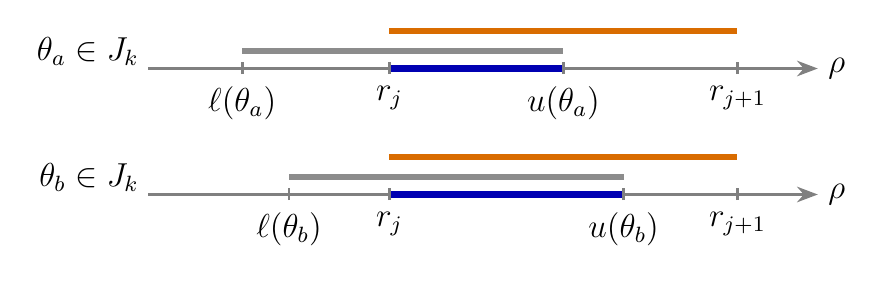
\begin{tikzpicture}[proofpic,x=1.7cm,y=1cm]
 \foreach \y/\leftend/\rightend/\ang in {0/.7/3.1/a,-1.6/1.05/3.55/b}{
  \begin{scope}[yshift=\y cm]
   \draw[rayline,->] (0,0)--(5,0) node[right] {$\rho$};
   \draw[black!45,line width=2.2pt] (\leftend,.22)--(\rightend,.22);
   \draw[orange!85!black,line width=2.2pt] (1.8,.48)--(4.4,.48);
   \draw[front] (1.8,0)--(\rightend,0);
   \foreach \xx/\lab in {\leftend/\ell(\theta_\ang),1.8/r_j,\rightend/u(\theta_\ang),4.4/r_{j+1}}{
    \draw[rayline] (\xx,-.07)--(\xx,.08);
    \node[below] at (\xx,-.1) {$\lab$};
   }
   \node[left] at (0,.22) {$\theta_\ang\in J_k$};
  \end{scope}
 }
\end{tikzpicture}
\caption{引理\ref{lem:structure}中的“截取方式不变”。灰线为单元区间，橙线为径向带，蓝线为二者交集。两条射线均满足 $\ell<r_j<u<r_{j+1}$，所以始终取 $L=r_j$、$U=u(\theta)$；蓝线长度可以变化，但端点的来源不变。}
\label{fig:lemma-clip}
\end{figure}

\section{覆盖定理与积分公式}
\begin{theorem}[几何切分的正确性与完备性]\label{thm:complete}
对于上述凸四边形与有限组同心圆，在每个存在单元交区间的 $J_k$ 内，令
\begin{equation}\label{eq:clip}
 L_{kj}(\theta)=\max\{\ell(\theta),r_j\},\qquad
 U_{kj}(\theta)=\min\{u(\theta),r_{j+1}\},\quad 0\leq j<m.
\end{equation}
则 $U_{kj}>L_{kj}$ 要么在整个 $J_k$ 内成立，要么处处不成立。保留前一种情况，定义
\begin{equation}\label{eq:cell}
 S_{kj}=\{\rho \bm{d}(\theta):\theta\in J_k,\ L_{kj}(\theta)<\rho<U_{kj}(\theta)\}.
\end{equation}
这些子区两两不交；将边界集合 $Z$ 加回后，恰好得到整个 $S$：
\begin{equation}\label{eq:union}
 S=\left(\mathop{\dot\bigcup}_{k,j:\,U_{kj}>L_{kj}} S_{kj}\right)\mathbin{\dot\cup}Z,
 \qquad |Z|=0.
\end{equation}
这里 $Z$ 为 $S$ 中位于单元边界、分割射线或所列圆周上的点；若原点属于 $S$，也将其计入 $Z$。$|Z|$ 表示二维面积。
\end{theorem}
\begin{proof}
引理 \ref{lem:structure} 保证端点来源及其与各圆半径的顺序不变。因此 $L_{kj},U_{kj}$ 各自的表达式固定；由 $\ell<u$、$r_j<r_{j+1}$ 及交叉比较关系不变，区间是否具有正长度也不变。

任取 $\bm{x}\in S\setminus Z$。其极坐标唯一对应一个 $J_k$ 和一个径向带 $(r_j,r_{j+1})$。由 $\bm{x}\in Q$ 及式 \eqref{eq:bounds}，必有
$L_{kj}<|\bm{x}|<U_{kj}$，故 $\bm{x}\in S_{kj}$。反过来，式 \eqref{eq:clip} 保证每个 $S_{kj}$ 均包含于 $S$。角区间和径向带均互不重叠，因此各子区两两不交。$Z$ 包含于有限条线段、有限条圆弧及一个点的并，面积为零。于是式 \eqref{eq:union} 成立。
\end{proof}

\textbf{为什么可以只检查角区间中点？}
定理说明：一个角区间与径向带的组合，不会在区间中途突然出现或消失。因此程序用中点决定是否保留该组合是充分的。\textbf{中点只用于判断是否为空，实际积分时的 $L_{kj}(\theta),U_{kj}(\theta)$ 仍须随角度计算，不能冻结为中点处的数值。}

\begin{figure}[htbp]
\centering
\begin{tikzpicture}[proofpic,x=1.5cm,y=1.5cm]
 \pgfmathsetmacro{\cutangle}{acos(3/3.2)}
 \fill[black!3] (1,-.35) rectangle (3,1.8);
 \draw[edge] (1,-.35) rectangle (3,1.8);
 \fill[blue!22] (2,0)--(3,0)--(3,{sqrt(1.24)})
  --(\cutangle:2) arc (\cutangle:0:2)--cycle;
 \draw[front] (0:2) arc (0:48:2);
 \draw[front] (0:3.2) arc (0:40:3.2);
 \draw[event] (0,0)--(3.6,0);
 \draw[event] (0,0)--(3.6,{3.6*sqrt(1.24)/3});
 \draw[rayline] (0,0)--(3.5,{3.5*tan(10)});
 \draw[line width=2.2pt,blue!70!black] (10:2)--(3,{3*tan(10)});
 \node[point,label=below:$O$] at (0,0) {};
 \node[point] at (10:2) {};
 \node[point] at (3,{3*tan(10)}) {};
 \node[above] at (2.45,.56) {$S_{kj}$};
 \node[left] at (48:2) {$r_j$};
 \node[above] at (40:3.2) {$r_{j+1}$};
 \node[below] at (3.55,0) {$\theta_k$};
 \node[right] at (3.5,{3.5*sqrt(1.24)/3}) {$\theta_{k+1}$};
 \node at (1.8,-.95) {（a）裁剪后的实际子区};
 \begin{scope}[xshift=8.7cm]
  \fill[blue!22] (0,0) rectangle (2.3,1.6);
  \draw[edge] (0,0) rectangle (2.3,1.6);
  \draw[rayline,->] (-.25,0)--(2.7,0) node[right] {$\theta$};
  \draw[rayline,->] (0,-.15)--(0,2) node[above] {$\eta$};
  \draw[front] (1.15,0)--(1.15,1.6);
  \node[left] at (0,0) {$0$};
  \node[left] at (0,1.6) {$1$};
  \node[below] at (0,0) {$\theta_k$};
  \node[below] at (2.3,0) {$\theta_{k+1}$};
  \node[above] at (1.15,1.65) {$\rho=U(\theta)$};
  \node at (1.15,-.55) {$\rho=L(\theta)$};
  \node at (1.15,-.95) {（b）参数矩形};
 \end{scope}
\end{tikzpicture}
\caption{径向裁剪与参数映射。图（a）取 $Q=[1,3]\times[-0.35,1.8]$、$r_j=2$、$r_{j+1}=3.2$，角区间为 $(0,\arccos(3/3.2))$。其内始终有 $L=2$、$U=3/\cos\theta$，蓝色区域恰为一个子区。每条径向线段通过 $\rho=L+\eta(U-L)$ 对应图（b）中的一条竖线。}
\label{fig:cell}
\end{figure}

\begin{corollary}[积分变换不引入几何近似]
对 $S$ 上绝对可积的函数 $f$，有
\begin{align}
 \int_S f(\bm{x})\dd A
 &=\sum_{k,j}\int_{\theta_k}^{\theta_{k+1}}
   \int_{L_{kj}(\theta)}^{U_{kj}(\theta)}
   f(\rho \bm{d}(\theta))\,\rho\dd\rho\dd\theta\label{eq:integral}\\
 &=\sum_{k,j}\int_{\theta_k}^{\theta_{k+1}}\int_0^1
   f(\rho(\theta,\eta)\bm{d}(\theta))\,
   \rho(\theta,\eta)(U_{kj}-L_{kj})\dd\eta\dd\theta,\label{eq:map}
 \intertext{其中求和仅遍历保留的子区，且}
 \rho(\theta,\eta)&=L_{kj}(\theta)+\eta\bigl(U_{kj}(\theta)-L_{kj}(\theta)\bigr).
 \nonumber
\end{align}
\end{corollary}
\begin{proof}
由定理 \ref{thm:complete}，零面积边界不影响可积函数的面积积分，故可逐区相加。极坐标面积元为 $\rho\dd\rho\dd\theta$；固定 $\theta$ 时，$\dd\rho=(U_{kj}-L_{kj})\dd\eta$，即得第二式。
\end{proof}

若所有核函数分段半径均已加入 $\{r_j\}$，每个子区内部就不会穿过核函数的径向分界。上式是精确恒等式；随后用高斯求积近似积分，才引入求积误差。继续细分子区可以提高求积精度，并不意味着几何分类仍有缺项。

\section{如何完整生成分割方向}
圆、边交点不需要分类求解。对每条边和每个正半径 $r$，求
\begin{equation}\label{eq:quadratic}
 |\bm{a}_i+t \bm{e}_i|^2=r^2
 \quad\Longleftrightarrow\quad
 |\bm{e}_i|^2t^2+2(\bm{a}_i\cdot \bm{e}_i)t+|\bm{a}_i|^2-r^2=0,
 \qquad 0\leq t\leq1.
\end{equation}
保留区间内的全部实根即可。二次方程给出直线与圆的全部交点，$0\leq t\leq1$ 又恰好限定在线段上，所以不会漏掉圆、边交点。重根对应相切，端点根对应圆过顶点；同一方向重复出现时只保留一次。

这也解释了几种容易担心的情况为何不需要另设算法：
\begin{itemize}
 \item \textbf{没有圆、边交点：}圆完全在单元内、单元完全在圆内或二者分离，均由式 \eqref{eq:clip} 的上下界自动区分；没有交点不等于没有积分区域。
 \item \textbf{相切、过顶点、多圆方向重合：}相应方向进入 $\mathcal E$；仅接触而没有面积的部分进入 $Z$，不会被误认为正面积子区。
 \item \textbf{圆心在边上或顶点上：}零向量不取辐角；沿边的非零方向由其他端点给出，原点本身归入 $Z$。引理 \ref{lem:edge} 已包含过圆心的边。
 \item \textbf{圆环交区不连通：}不同连通部分可落在不同角区间中，式 \eqref{eq:union} 仍逐一覆盖；证明只使用四边形的凸性，不要求圆环交区连通。
\end{itemize}

对于三维源点到单元平面的距离 $h$，空间波前距离 $R$ 满足 $R^2=h^2+\rho^2$。因此 $R>h$ 时加入平面半径 $\sqrt{R^2-h^2}$；$R=h$ 时退化为原点，$R<h$ 时没有平面交线。由此，空间波前问题完整归结为本文的同心圆问题。

\paragraph{与现有程序的对应。}
\texttt{planeCells} 收集顶点和圆、边交点的角度，并用角区间中点筛选子区；\texttt{ray} 实现式 \eqref{eq:ray}--\eqref{eq:bounds}；径向映射实现式 \eqref{eq:clip} 和 \eqref{eq:map}。本文证明了这套几何规则在精确实数运算下的完备性；浮点求根、角度合并的容差仍需按数值精度核验，不能由几何证明替代。

\end{document}
